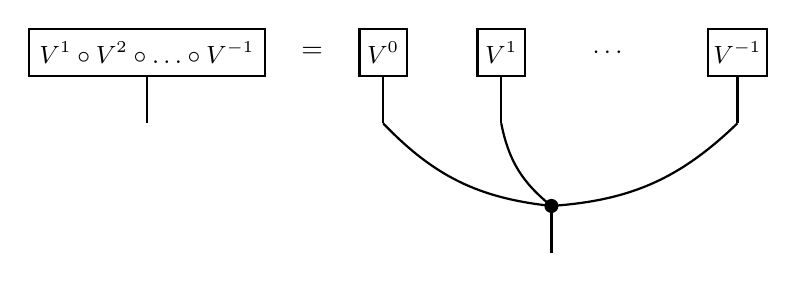
\begin{tikzpicture}[scale=0.3,thick] % , baseline = -3.5pt


\begin{scope}[shift={(-10,0)}]

\draw (-3,1) rectangle (7,3);
\node[anchor=center] (text) at (2,2) {\small $V^1\circ V^2 \circ \ldots \circ V^{\atomorder-1}$};
\draw (2,-1)--(2,1) node[midway,right] {\tiny $\catvariable$};

\node[anchor=center] (text) at (9,2) {${=}$};

\end{scope}



\draw (1,1) rectangle (3,3);
\node[anchor=center] (text) at (2,2) {\small $V^0$};
\draw (2,-1)--(2,1) node[midway,right] {\tiny $\catvariable$};


\begin{scope}[shift={(5,0)}]

\draw (1,1) rectangle (3,3);
\node[anchor=center] (text) at (2,2) {\small $V^1$};
\draw (2,-1)--(2,1) node[midway,right] {\tiny $\catvariable$};

\end{scope}

\node[anchor=center] (text) at (11.5,2) {\small $\cdots$};


\begin{scope}[shift={(15,0)}]

\draw (0.75,1) rectangle (3.25,3);
\node[anchor=center] (text) at (2,2) {\small $V^{\atomorder-1}$};
\draw (2,-1)--(2,1) node[midway,right] {\tiny $\catvariable$};

\end{scope}


\draw[fill] (9.125,-4.5) circle (0.25cm);

\draw (9.125,-4.5) to[bend right=-20] (2,-1); 
\draw (9.125,-4.5) to[bend right=-20] (7,-1); 
\draw (9.125,-4.5) to[bend right=20] (17,-1); 

\draw (9.125,-4.5) -- (9.125,-6.5) node[midway,right] {\tiny $\catvariable$};;

\end{tikzpicture}